\section{Auswertung}
Im Folgenden sollen die Messergebnisse analysiert werden und die relevanten Größen aus der Theorie berechnet werden. \\
Die Werte für die beiden Temperaturen $T_1$ und $T_2$ sowie die Drücke $p_a$ und $p_b$ sind in Tablle \ref{tab: tempdruck} aufgetragen.
\FloatBarrier
\begin{table} 
 \centering 
 \begin{tabular}{S S S S S } 
 \toprule  
{Zeit in $\si{\second}$} & {$T_1$ in $\si{\kelvin}$} & {$p_b$ in $\si{\bar}$} & {$T_1$ in $\si{\kelvin}$} & {$p_b$ in $\si{\bar}$} \\ 
\midrule  
 0 & 293.75 & 5.25 & 294.05 & 5.20 \\ 
60 & 295.05 & 7.25 & 294.15 & 2.40 \\ 
120 & 296.65 & 7.50 & 294.15 & 2.90 \\ 
180 & 298.15 & 8.00 & 294.05 & 3.00 \\ 
240 & 300.45 & 8.50 & 294.05 & 3.10 \\ 
300 & 302.75 & 9.00 & 294.05 & 3.20 \\ 
360 & 305.25 & 9.50 & 293.95 & 3.20 \\ 
420 & 307.55 & 10.00 & 293.45 & 3.20 \\ 
480 & 309.65 & 10.50 & 291.45 & 3.20 \\ 
540 & 311.65 & 11.00 & 288.55 & 3.20 \\ 
600 & 313.55 & 11.25 & 285.95 & 3.20 \\ 
660 & 315.55 & 11.75 & 283.95 & 3.22 \\ 
720 & 317.15 & 12.00 & 282.75 & 3.22 \\ 
780 & 318.75 & 12.50 & 281.75 & 3.22 \\ 
840 & 320.35 & 13.00 & 280.95 & 3.20 \\ 
900 & 321.75 & 13.25 & 280.45 & 3.20 \\ 
960 & 323.05 & 13.50 & 280.05 & 3.20 \\ 
\bottomrule 
 \end{tabular} 
 \caption{Temperaturen und Drücke} 
 \label{tab: tempdruck} 
  \end{table}
\FloatBarrier
Der zeitliche Verlauf der Temperaturen ist in den Abbildungen (...) dargestellt. Hierbei wurde mittels der Python Bibliothek $Scipy$ eine %... ersetzen, scipy am besten mit \emph{} setzen
Regression an eine Funktion der Form $T_i = A t^2 + B t + C$ bestimmt. Um im späteren Verlauf eine präzisere Aussage über den Temperaturverlauf
von $T_2$ zu gewährleisten, wurde selbiges für den Zeitraum nach $t_0 = 360 \si{\second}$ erneut durchgeführt ($T_2*$). In der Diskussion wird hierauf näher eingegangen. Die entsprechenden
Parameter sind in Tabelle \ref{tab: regress} zu finden. \\

\begin{table} 
 \centering 
 \begin{tabular}{S S S S } 
 \toprule  
{Funktion} & {$A$} & {$B$} & {$C$} \\ 
\midrule  
 $T_1$ & $\num{-6.77 \pm 1.67}$ & $\num{3.86\pm 0.18}$ & $\num{292.45 \pm 0.39}$ \\ 
$T_2$ & $\num{-10.98 \pm 4.88}$ & $\num{-0.67 \pm 0.52}$ & $\num{295.52 \pm 1.13}$ \\ 
$T_2*$ & $\num{32.83 \pm 7.24}$ & $\num{-6.91\pm 0.96}$ & $\num{315.85 \pm 3.01}$ \\ 
\bottomrule 
 \end{tabular} 
 \caption{Regressionsparameter} 
 \label{tab: regress} 
  \end{table}
\begin{figure}
  \centering
  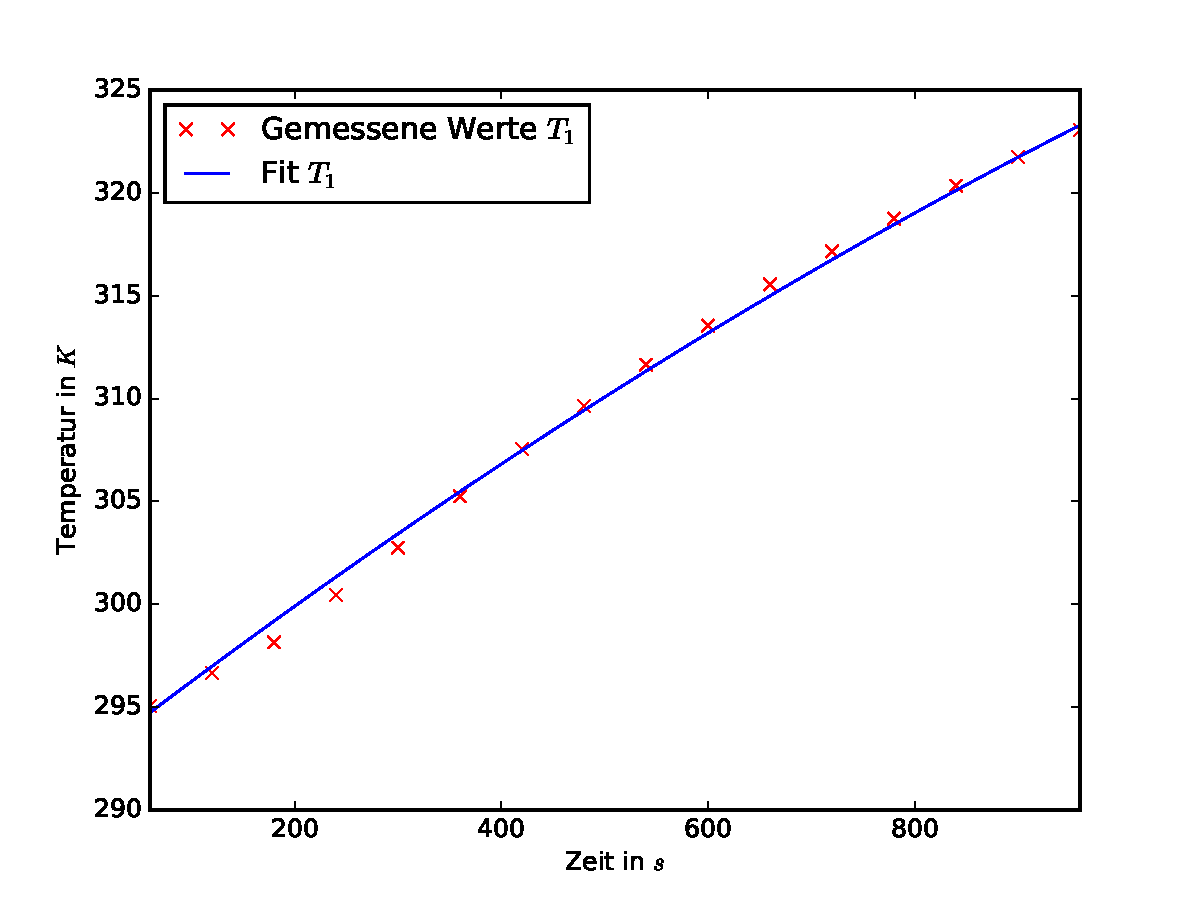
\includegraphics[width = 14cm]{tabs/plot1.pdf}
  \caption{Temperaturverlauf $T_1$}
  \label{fig: plot1}
\end{figure}

\begin{figure}
  \centering
  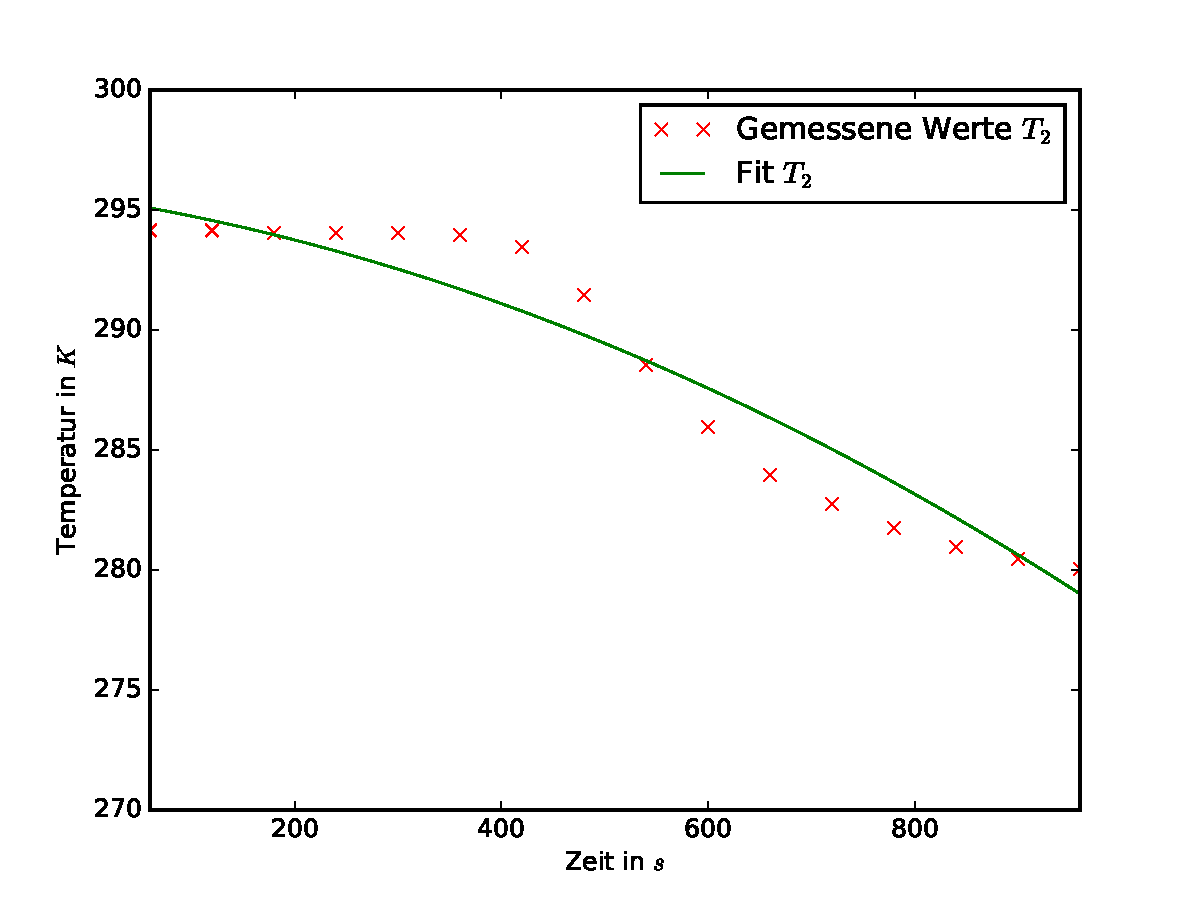
\includegraphics[width = 14cm]{tabs/plot2_1.pdf}
  \caption{Temperaturverlauf $T_2$}
  \label{fig: plot2}
\end{figure}

\begin{figure}
  \centering
  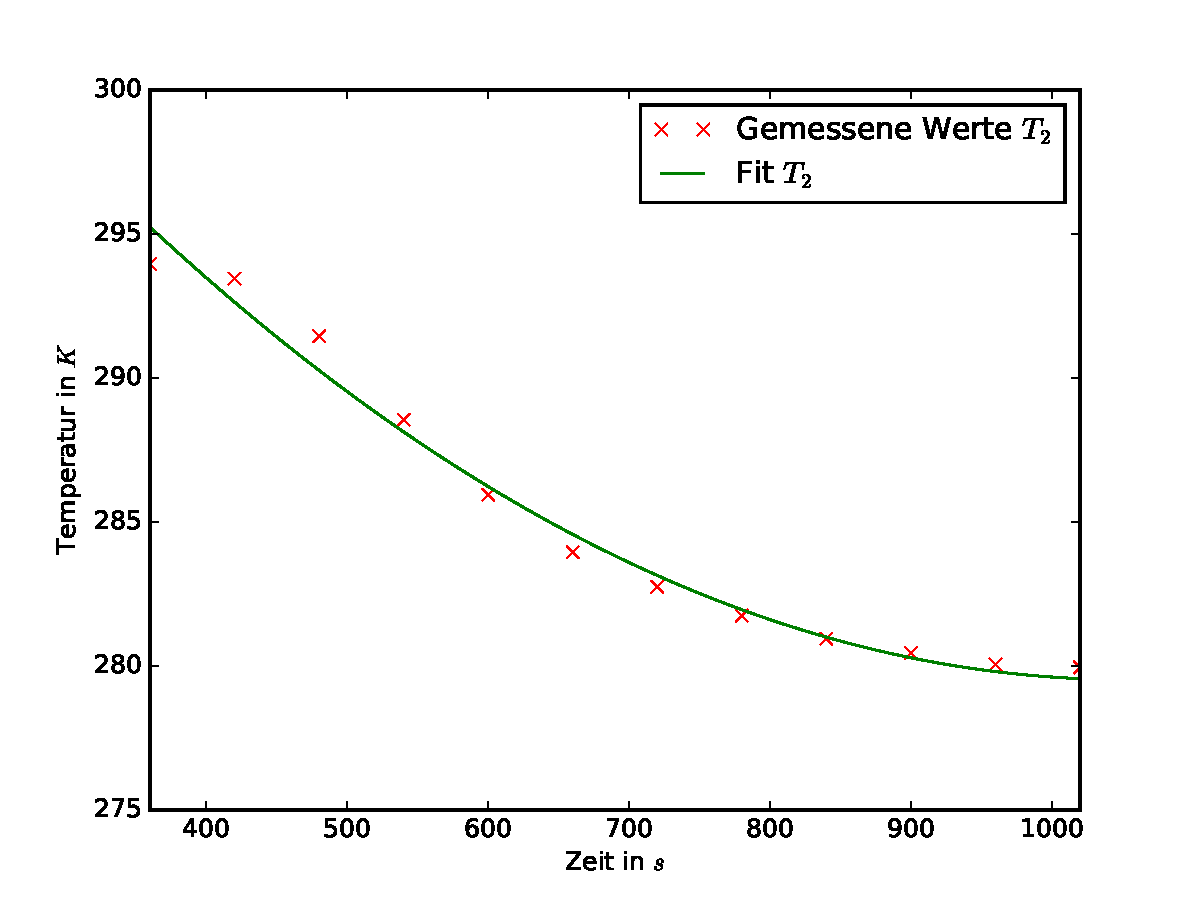
\includegraphics[width = 14cm]{tabs/plot2_2.pdf}
  \caption{Temperaturverlauf $T_2$ für $t > 360 \si{\second}$}
  \label{fig: plot2*}
\end{figure}


Die gefundenen Regressionskurven erlauben es, die Differentialquotienten $\frac{dT_1}{dt}$ und $\frac{dT_2}{dt}$ zu berechnen. Die Werte für vier verschiedene  Zeiten sind %\mathup
in Tabelle \ref{tab: dTdt} aufgetragen, die entsprechenden Fehler $o_{dT_i}$ ergeben sich über die Gaußsche Fehlerfortpflanzung. Hierbei wurden die Zeiten $t > t_0$ gewählt, sodass die Kurve aus Abbildung \ref{fig: plot2*} verwendet werden konnte. %%\mathup

\subsection{Güteziffer}

Mittels des Zusammenhangs
\begin{equation}
  \nu_{real} = (m_1 c_w + m_k c_k) \frac{dT_1}{dt} \frac{1}{P} % %\mathup
\end{equation}
wurde die reale Güteziffer $\nu_{real}$ berechnet. Hierbei entsprechen $m_k c_k = 660 \si{\joule \per \second}$ und $c_1 c_W$ den Wärmekapzitäten von Apparatur und Wasser. Die Masse $m_1 = V_1 \cdot \rho_w$ ergibt sich mit
der Dichte des Wassers $\rho_w \approx 1000 \si{\kilo \gram \per \meter ^3}$  und der entsprechenden Füllmenge $V_1 = 3 l$. Der Wert $c_w = 4182\si{\joule \kilo \gram^{-1} \kelvin^{-1}}$ wurde der Literatur \cite{demtröder} entnommen. %^3 durch \cubic ersetzen ->\per\cubic\meter, ^{-1} durch \per ersetzen
Da hier lediglich die Größe $\frac{dT_1}{dt}$ fehlerbehaftet ist, berechnet sich der Fehler zu: %\mathup
\begin{equation}
  o_{\nu_{real}} = \left| const \right| \cdot o_{dT_1} %\mathup
  \label{eq: errorconst}
\end{equation}

Die Ergebnisse der Rechnung, sowie die ideale Güteziffer $\nu_{ideal}$ (formel) (fehlerunbehaftet) sind in Tabelle \ref{tab: dTdt} aufgetragen.
\begin{table} 
 \centering 
 \begin{tabular}{S S S } 
 \toprule  
{Zeit in $\si{\second}$} & {$\frac{dT_1}{dt}$ in $\si{\kelvin \per \second}$} & {$\frac{dT_2}{dt}$ in $\si{\kelvin \per \second}$} & {$\nu_{real}$} \\ 
\midrule  
 0 & $\num{ 3.86 \pm 0.18 }$ & $\num{ -0.67 \pm 0.52 }$ & $\num{ 51014.25 \pm 2336.66 }$ \\ 
60 & $\num{ -808.83 \pm 200.88 }$ & $\num{ -1317.96 \pm 585.31 }$ & $\num{ -61036.66 \pm 15159.09 }$ \\ 
120 & $\num{ -1621.52 \pm 401.76 }$ & $\num{ -2635.26 \pm 1170.61 }$ & $\num{ -118965.82 \pm 29475.99 }$ \\ 
180 & $\num{ -2434.22 \pm 602.64 }$ & $\num{ -3952.55 \pm 1755.92 }$ & $\num{ -173763.66 \pm 43019.02 }$ \\ 
240 & $\num{ -3246.91 \pm 803.53 }$ & $\num{ -5269.85 \pm 2341.23 }$ & $\num{ -219890.81 \pm 54417.22 }$ \\ 
300 & $\num{ -4059.60 \pm 1004.41 }$ & $\num{ -6587.14 \pm 2926.53 }$ & $\num{ -268055.69 \pm 66320.98 }$ \\ 
360 & $\num{ -4872.30 \pm 1205.29 }$ & $\num{ -7904.44 \pm 3511.84 }$ & $\num{ -313871.07 \pm 77644.07 }$ \\ 
420 & $\num{ -5684.99 \pm 1406.17 }$ & $\num{ -9221.73 \pm 4097.15 }$ & $\num{ -366224.39 \pm 90584.75 }$ \\ 
480 & $\num{ -6497.69 \pm 1607.05 }$ & $\num{ -10539.03 \pm 4682.45 }$ & $\num{ -412540.53 \pm 102032.28 }$ \\ 
540 & $\num{ -7310.38 \pm 1807.93 }$ & $\num{ -11856.33 \pm 5267.76 }$ & $\num{ -459718.39 \pm 113693.11 }$ \\ 
600 & $\num{ -8123.07 \pm 2008.81 }$ & $\num{ -13173.62 \pm 5853.07 }$ & $\num{ -508404.23 \pm 125726.98 }$ \\ 
660 & $\num{ -8935.77 \pm 2209.69 }$ & $\num{ -14490.92 \pm 6438.37 }$ & $\num{ -559268.83 \pm 138299.67 }$ \\ 
720 & $\num{ -9748.46 \pm 2410.58 }$ & $\num{ -15808.21 \pm 7023.68 }$ & $\num{ -610133.43 \pm 150872.37 }$ \\ 
780 & $\num{ -10561.15 \pm 2611.46 }$ & $\num{ -17125.51 \pm 7608.98 }$ & $\num{ -660998.03 \pm 163445.07 }$ \\ 
840 & $\num{ -11373.85 \pm 2812.34 }$ & $\num{ -18442.80 \pm 8194.29 }$ & $\num{ -715252.45 \pm 176855.95 }$ \\ 
900 & $\num{ -12186.54 \pm 3013.22 }$ & $\num{ -19760.10 \pm 8779.60 }$ & $\num{ -773728.10 \pm 191310.52 }$ \\ 
960 & $\num{ -12999.23 \pm 3214.10 }$ & $\num{ -21077.39 \pm 9364.90 }$ & $\num{ -833339.20 \pm 206045.76 }$ \\ 
\bottomrule 
 \end{tabular} 
 \caption{Differenzenquotienten und reale Güteziffer} 
 \label{tab: dTdt} 
  \end{table}

\subsection{Massendurchsatz und Mechanische Leistung}
Zur Bestimmung des Massendurchsatzes $\frac{dm}{dt}$ wird zunächst die Verdampfungswärme $L$ benötigt. Hierzu wird der aus $V203$ \cite{anleitung203} bekannte Zusammenhang des Druckverlaufs für $p_b$ in Abhängigkeit von der Temperatur%%\mathup
\begin{equation}
  p_b = p_0 \exp{-\frac{L}{R T_1}} %Klammern setzen
\end{equation}
ausgenutzt. Durch einmaliges Anwenden des Logarithmus erhält man einen linearen Zusammenhang der Form:
\begin{equation}
  \log{p_b} = \log{p_0} -\frac{L}{R} \cdot \frac{1}{T_1} 
\end{equation}
Durch halb-logarithmisches Auftragen der Werte für $p_b$ gegen die Reziproken der Temperatur $T_1$ (siehe Abb. \ref{fig: plot3}) kann also mit Hilfe einer lineare Regression die Steigung $-\frac{L}{R}$ ermittelt werden.
Steigung und zugehöriger Fehler berechnen sich mit:
\begin{equation}
  m= \frac{\left( N  (\sum x_i y_i) - (\sum x_i)(\sum y_i)\right)}{N (\sum x_i^2)- (\sum x_i)^2 }    \quad   o_m=\frac{N o_y^2}{N (\sum x_i^2)- (\sum x_i)^2 }
\end{equation}
Es ergibt sich:
\begin{equation}
  -\frac{L}{R} =  (-2228.58 \pm 111.63) \si{\kelvin}
\end{equation}

\begin{figure}
  \centering
  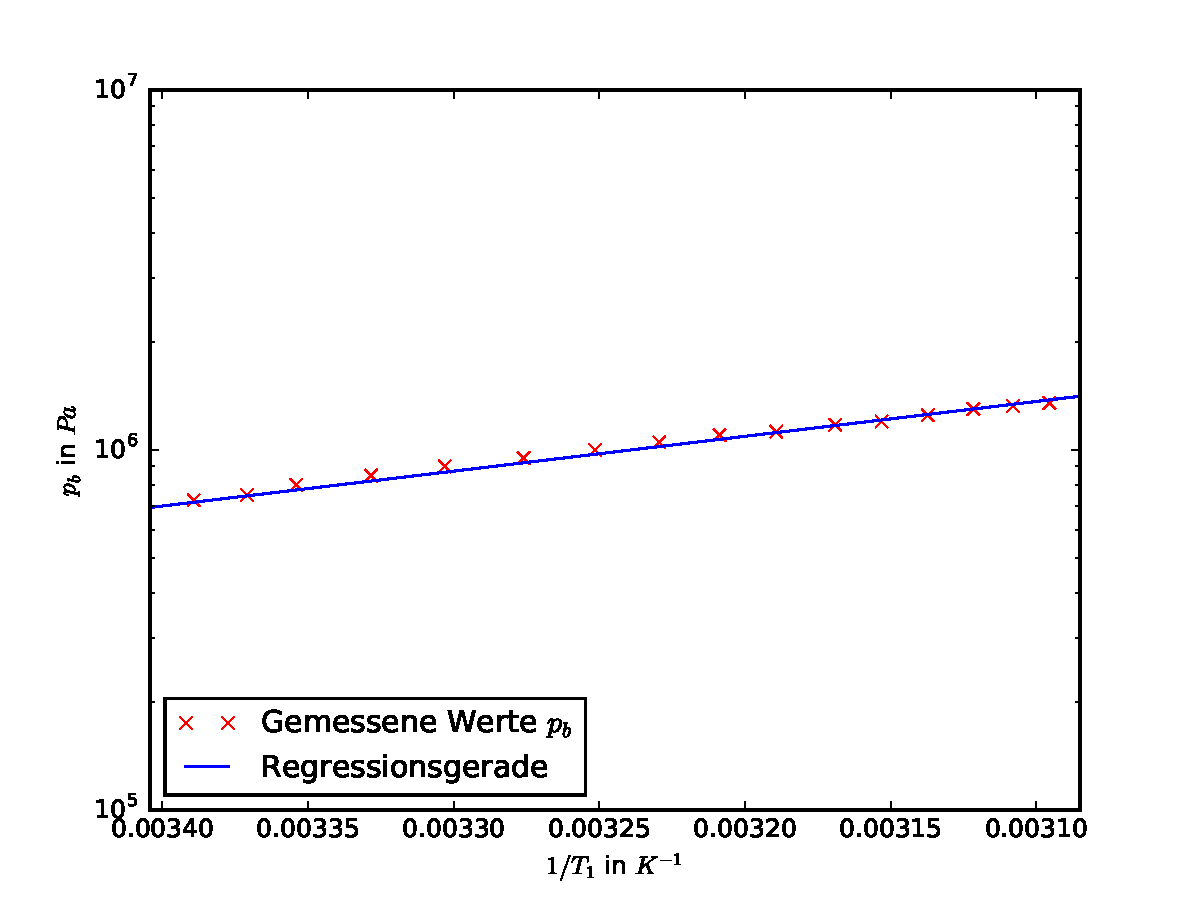
\includegraphics[width = 14cm]{tabs/plot3.pdf}
  \caption{Regression der Druckkurve}
  \label{fig: plot3}
\end{figure}

Mit der allgemeinen Gaskonstante $R = 8.314\si{\joule \mol^{-1} \kelvin^{-1}}$ ergibt sich $L$  mit \eqref{eq: errorconst} zu: %^{-1} mit \per ersetzen
\begin{equation}
  L = (1.85 \pm 0.09)\cdot 10^{4} \si{\joule \mol^{-1}} %^{-1}
\end{equation}
Der Massendurchsatz berechnet sich nun mit:
\begin{equation}
  \frac{dm}{dt} = (m_2 c_w + m_k c_k)\frac{dT_2}{dt} \frac{1}{L}
\end{equation}
Mit der identischen Wärmekapazitäten $m_2 c_w$ und $m_k c_k$ wie oben. Die berechneten Werte sind in Tabelle \ref{tab: dmdtNmech} aufgetragen, der relative Fehler berechnet sich gemäß der üblichen Formel
für Produkte und Quotienten:
\begin{equation}
  \frac{o_{dm}}{\left| dm \right|} = \left| const \right| \sqrt{\left(\frac{o_{dT_2}}{\left| dT_2 \right|}\right)^2 + \left(\frac{o_{L}}{\left| L \right|}\right)^2} %%\mathup
\end{equation}
Des Weiteren wurde mittels der molaren Masse des Gases $120,91 \si{g \mol ^{-1}}$ \cite{demtröder} umgerechnet in die Einheit $\si{\gram \per \second}$. \\%g? (wenn gramm dann \gram) s
Abschließend soll nun noch die mechanische Leistung des Kompressors errechnet werden. In Formel (x) kann $\frac{1}{\rho}$
näherungsweise mit der idealen Gasgleichung bestimmt werden.
\begin{equation}
  pV = nRT \Leftrightarrow  \frac{1}{\rho} = \frac{\rho_0 T_0 p_a}{T_2 p_0}
\end{equation}
Mit den aus der Versuchsanleitung \cite{anleitung206} entnommenen Konstanten des Gases $CI_2F_2C$. Die entsprechenden Mittelwerte befinden sich in Tabelle \ref{tab: dmdtNmech}.





\begin{table}
 \centering
 \begin{tabular}{S S S }
 \toprule
{Zeit in $\si{\second}$} & {$\frac{dm}{dt}$ in $\si{\gram \per \second}$} & {$N_{mech}$ in $\si{\watt}$}  \\
\midrule

360  & $\num{ 3.88 \pm 0.96 }$ & $\num{ 77.49 \pm 19.09 }$ \\

540  & $\num{ 2.87 \pm 1.07 }$ & $\num{ 64.45 \pm 24.02 }$ \\

720  & $\num{ 1.86 \pm 1.22 }$ & $\num{ 43.84 \pm 28.66 }$ \\

900  & $\num{ 0.85 \pm 1.39 }$ & $\num{ 21.64}^{+35.20}_{-21.64} $ \\





\bottomrule
 \end{tabular}
 \caption{Massendurchsatz und Kompressorleistung}
 \label{tab: dmdtNmech}
  \end{table}

